\chapter{Future Work Plan}
\label{chap:future}

In this chapter we break down the the four main objectives we have identified in Chapter \ref{chap:aimsObj} into small working packages, present mile-stones and holidays, relevant conferences, papers we want to publish (either conference or journal). A Gantt-Chart, reflecting all the details is found at the end of this chapter in Figure \ref{fig:gantt}.

\section{Planned Papers}
We plan for three papers with at least one of them to be submitted to a journal.

\subsection{FrABS - Towards pure functional programming in ABS}
This paper will present the pure functional approach to ABS we have taken and outlined in Appendix \ref{app:frABS}. It will describe the combination of FRP \& ABS, the EDSL built on top and gives some examples of specification and implementation of the SIRS and Sugarscape model.

\subsection{Will it Equilibrate? Reasoning in pure functional ABS}
In this paper we will discuss the verification method we have developed using our FrABS implementation and QuickCheck. We describe the decentralized bilateral bartering process of the Sugarscape model and verify it.
-> purely reasoning about the bilateral trading in sugarscape.
	-> explain bilateral decentralized bartering
	-> general equilibrium theory
	-> give reason in code for the failure of reaching equilibrium

\subsection{Deterministic Concurrency in ABS through Transactional Functional Reactive Agents}
	-> following the hypothesis that STM is the real unique thing which can be only done in Haskell and not in Java we ask if and how we can leverage on it?
	-> introducing the concept of STM to ABS to support concurrent ABS
	-> concurrency leads to non-reproducibility, is it still of use? e.g. what about replications in this context?
	-> non-reproducible results are in some kind of way useless, can we find another definition of reproducibility? e.g. when using yampas time-semantics? or when using 

\section{Years Overview}

\subsection{1st Year}
In the first year, all is about orientation, experimenting and finding out what the PhD is \textit{really} going to be about. The aim is to have a good working prototype of the library with a few good examples - including SugarScape and Agent\_Zero ready. 

\subsection{2nd Year}
In the second year, the focus will be on \textit{verification}. Using the FrABS library and QuickCheck we will research how far we can go into formalizing model-specifications and how well we can do verification. 

\subsection{3rd Year}
Tocus on cleaning up the research and writing the final thesis. The plan is to start the writing of the final thesis around April 2019 with a 5-months writing-window and to submit on-time at end of September 2019.

\section{Conferences}
\begin{itemize}
	\item \textbf{Multi-Agent Systems AAMS} - General Multi-Agent Systems and Agent-Based Modelling \& Simulation, Deadline in November
	\item \textbf{Social Simulation Conference SSC} - New Methods and models in simulation, Deadline in March
	\item \textbf{Symposium on Trends in Functional Programming} - Functional programming stuff, Deadline in May
\end{itemize}

\section{Mile-Stones}
\begin{itemize}
	\item 2017 31st March - finished and submit Paper 
	\item 2017 18th June - Finished writing 1st year report 
	\item 2017 21st July - 1st Annual Review
	\item 2017 October - 2nd year starts
	\item 2018 May - Submit Paper on FrABS
	\item 2018 October - 3rd year starts
	\item 2019 February - Submit Paper on Verification
	\item 2019 April - Begin of thesis-writing
	\item 2019 September - Submit Thesis
	\item 2019 30th September - official end of PhD
	\item 2020 30th September - end of pending-period
\end{itemize}


\label{app:gantt}
\begin{landscape}
	\begin{figure}
		\label{fig:gantt}
  		\caption{Gantt-Chart for remaining PhD}
  		\centering
  		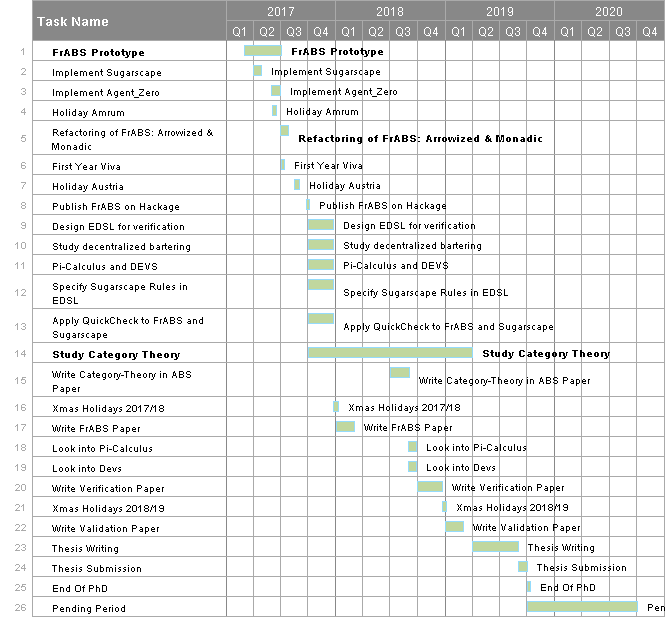
\includegraphics[width=1.2\textwidth]{./charts/gantt.png}
	\end{figure}
\end{landscape}